\chapter{Physical Organization}

We said at the beginning that a DBMS is made out of multiple layers: an \textbf{external} layer, a \textbf{logic} layer and a \textbf{physical} layer. In the previous chapters we always dealt with the logical later, now we'll focus on the physical layer.
\nwl
We know that in a computer there are two types of memory: \textbf{volatile} and \textbf{non-volatile}. Some examples of volatile memory are the CPU registers, the cache and the central storage, while some examples of non-volatile memory are HDDs (Hard Disks Drive) or SSDs (State Solid Drive). The examples that we gave for volatile memory represent elements with a high-speed memory, but they are costly and limited in the capacity; regarding non-volatile memory instead, we have slower memory, but it's cheaper and has less limits regarding the capacity.
\nwl
In a DBMS, the physical data is stored on the secondary storage such as HDDs and SSDs, while the buffer and the code of the DBMS is stored in a buffer, which is considered as part of the primary memory.

\begin{center}
    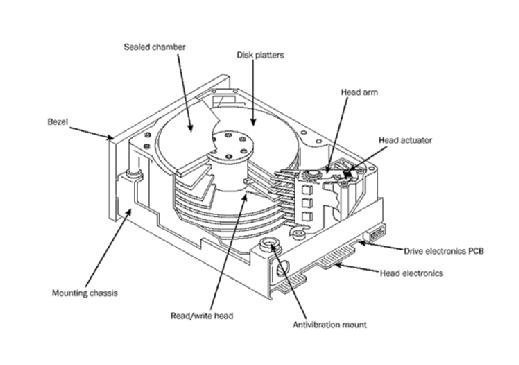
\includegraphics[scale = 0.7]{assets/images/image1.jpg}
    \\
    View of an HDD
\end{center}

How do HDDs work? They have a set of \textbf{disks} (or \textbf{platters}), which are covered in a magnetic dust. The platters rotate on a spindle at a constant speed. Via the use of some arms and some heads, the data can be read and write from/to the hardisk. Hardisks are also called \textbf{D}irectly \textbf{A}ccessible \textbf{S}torage \textbf{D}evices (\textbf{DASDs}).
\nwl
Whenever we have to read from a disk, we have to locate the sector on which the data is written: this implies that we need some time in order to position the actuator (called \textbf{seek time}) and wait until the disk rotates enough to make the sector arrive under the head (we call such delay the \textbf{rotation delay}).

\begin{definition}{Seek time and Rotation delay}
    We call \textbf{seek time} the time needed to position the head on the correct track of the disk.
    \nwl
    The \textbf{rotation delay} (\textbf{ROT}) is the delay given by the waiting that the disk rotates until the required disk sector is brought under the read/write head.
\end{definition}

There are some other timings that we consider:
\begin{itemize}
    \item [1)] \textbf{transfer time} (\textbf{TR}): it's the time needed to transfer a quantity of data from/to the disk. It's given by the \textbf{block size}, by the \textbf{density} of the \textbf{magnetic particles} and on the \textbf{rotation speed} of the \textbf{disks};
    \item [2)] \textbf{service time}: it's the sum between the \textbf{seek time}, the \textbf{rotational delay} and the \textbf{transfer time};
    \item [3)] \textbf{response time}: it's the sum between \textbf{service time} and \textbf{queuing time}.
\end{itemize}

Some other two important timings are:
\begin{itemize}
    \item [1)] \textbf{Random Block Access Time} ($T_{\text{rba}}$): it's the expected time to read/write on a disk regardless of the previous read/write operations
    \[ T_{\text{rba}} \eq \text{Seek} \; + \; \frac{\text{ROT}}{2} \; + \; \frac{\text{BS}}{\text{TR}} \]
    \item [2)] \textbf{Sequential Block Access Time} ($T_{\text{sba}}$): it's the expected time to sequentially retrieve the disk block with the read/write head already in place
    \[ T_{\text{sba}} \eq \frac{\text{ROT}}{2} + \frac{\text{BS}}{\text{TR}}\]
\end{itemize}

With \textbf{BS} we mean the \textbf{B}lock \textbf{S}ize. How can we have the most optimal storing result? We need a system for which the organization on the various tracks and cylinders minimizes as much as possible the \textbf{seek time} and, partially, the \textbf{rotation delay}; we also want to minimize as much as possible the accesses to different blocks. We can't have everything all at once, some trade-offs must be made. We will focus here on the physical organization of structured, relational data.

\section{Primary File Organization Methods}

At a physical level, the database consists of a set of various \textbf{files}; each file can be organized as a set of different \textbf{pages}, where each page has a fixed length (of usually 4KB). Each page can store several \textbf{records}, where a record consists of different \textbf{fields}, with either a fixed or variable size. Each field represents an attribute value. There are various ways for which we can find the records in the disk:
\begin{itemize}
    \item via \textbf{linear search}, where each record is stored and retrieved depending on a key;
    \item via \textbf{hashing} or \textbf{indexing}, where the location on the disk is specified by its relationship with the record search key. Such method has an improved performance in contrast to the linear search, since we have a direct access to the location where the record is stored;
    \item via the organization and the \textbf{type of files}: there could be \textbf{heap files}, \textbf{sequential files}, \textbf{random files}, \textbf{indexed sequential files} or \textbf{lists of data}.
\end{itemize}

\subsection{Heap file organization}

Such type of file is the basic of primary files organization. Each time a new record has to be inserted in a file, it gets added at the \textbf{end} of such file. Here we have \textbf{no relationship} between the record's attributes and their physical location, so the only option for retrieval is \textbf{linear search}. For a file with a number of blocks (\textbf{NBLK}), it usually takes $\nicefrac{\text{NBLK}}{2}$ time to find the record according to the given key. If the search key is not unique, then the whole file has to be scanned.

\subsection{Sequential file organization}

In this kind of file, the data is stored in an \textbf{ascending/descending order} depending on the search key. It's way more efficient to access the records in a specified order rather than not knowing where we have to look for. Although the data is stored in such way, we still access to the records with a linear search, but we have a \textbf{stopping} criterion: we stop whenever a key is higher/lower than the one needed. In order to have a more effective search method, we can use \textbf{binary search}: for a unique key $K$, with values $K_i$, we retrieve the record with the key value $K_\mu$.

\begin{question}
    \texttt{
        \begin{itemize}
            \item Selection criterion: record with search value $k_\mu$
            \item Set $l = 1$ and $h$ as the number of blocks in a file, supposing that the records are stored in an ascending order with respect to the search key $K$
            \item Repeat until $h \geq 1$:
            \begin{itemize}
                \item Set $i \eq \frac{(1 + h)}{2}$, rounded to the nearest integer
                \item Retrieve block $i$ and examine key values $K_j$ of records in block $i$
            \end{itemize}
            \item if any $K_j \eq K_\mu$, then the record is found and we can exit
            \item else if $K_\mu > \text{all } K_j$, then continue with $l \eq i + 1$
            \item else if $K_\mu < \text{all } K_j$, then continue with $h \eq i - 1$
            \item else the record is not in the file.
        \end{itemize}
    }
\end{question}

\section{Exercises}

\begin{exercise}
    Assume we have a file with \textbf{250.000} records, each of them of size \textbf{300} bytes, \textbf{75} of which for the key field. Each block is of size \textbf{1024} bytes. A block pointer is \textbf{4} bytes.
    \begin{itemize}
        \item [A)] If we use a hash organization with 1200 buckets, how many blocks do we need for the bucket directory?
        \item [B)] How many blocks do we need for the buckets, assuming a uniform distribution of records into buckets?
        \item [C)] Still assuming a uniform distribution of records, what is the average number of accesses needed to find a record in the file?
        \item [D)] How many buckets should we create to have instead an average number of accesses less or equal 10, still assuming a uniform distribution of records in the buckets?
    \end{itemize}
\end{exercise}